\begin{figure*}[ht!]
\centering
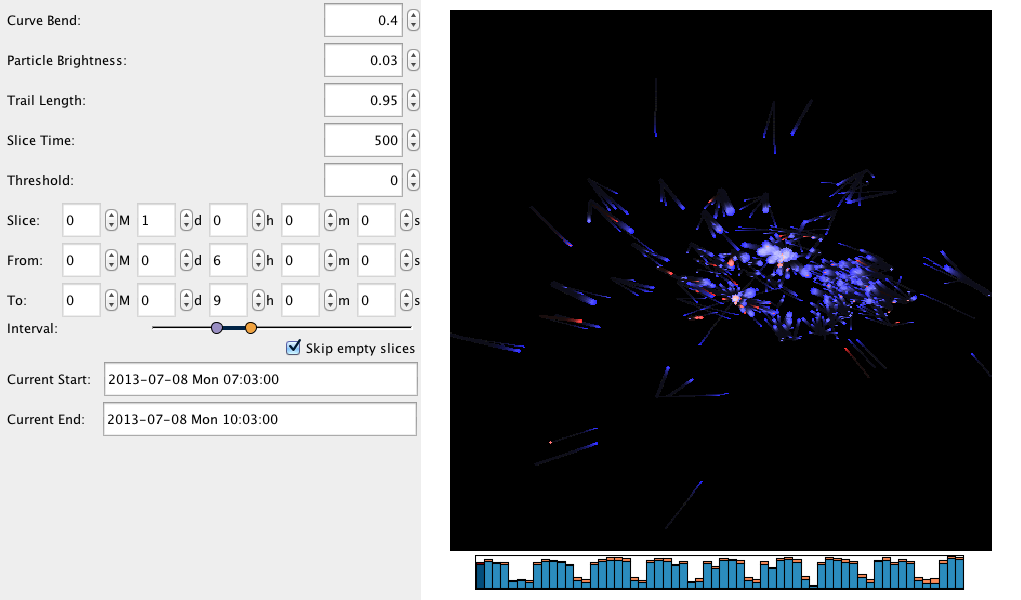
\includegraphics[width=0.9\linewidth]{images/tool.png}
\caption{The tool is split in three parts. On the right side is the
dot visualization. On the bottom right is the bar chart representation.
On the left is the control panel,
where the user can define the excursion of the trips, the brightness of
the dots, the length of the trails, the animation speed of the slices
and the threshold to remove dots that are too small.
With the spinners below this, the user can define the length of a slice and
the start and end of the relevant window.
The relevant window can also be edited by using the sliders below.
The user has also the option to skip slices that contain no trips, however
this only occurs when the duration of the slice is chosen very short.
The text fields at the bottom show the start and the end time of the
currently displayed relevant window.
}
\label{fig:tool}
\end{figure*}

\section{Related Work}
\label{sec:rel}
Multiple approaches have been used
to visualize origin-destination data with temporal features.

Rae~\cite{Rae2009} use heat-maps based on
the density of migration flows of cities in the UK.
The user can also select a city to see its flow
in a node-link representation.
By computing density based clusters,
Guo~\etal\cite{Guo2012} define regions
to show the net-flow of taxis in Hong Kong
as choropleth maps.
A kernel density representation shows
the distribution of destinations.
A multi-color kernel density representation is
used by Ferreira~\etal\cite{Ferreira2013}
to show the distribution of
origins and destinations of taxi trips in New York.

Guo~\etal\cite{Guo2006} use an origin-destination matrix
to show companies relocating within the US.
Rows and columns can be reordered to identify clusters
and patterns, but provide no spatial context.
Also, the resolution of origins and destinations is limited
to states due to the use of a matrix.
In order to address the lack of spatial context
Wood~\etal\cite{Wood2002} explore nested matrices
that are laid over a geographic map.
Every cell of the matrix aggregates the origins
of the geographic map and contains
a second matrix showing aggregated destinations of
a smaller scale version of the map.

Becker~\etal\cite{Becker1995} compare
origin-destination matrices to node-link representations
and propose an animated dynamic node-link representation
where the user can define time intervals to aggregate the data,
set thresholds to limit the number of visible links,
and choose the regions that are displayed.

The use of animation can make keeping track of changes
difficult (Tversky~\etal\cite{Tversky2002}).
However, animation can be used to
identify trends (Heer and Robertson~\cite{Heer2007},
and Robertson~\etal\cite{Robertson}) and
patterns (Griffin and MacEachren\cite{Griffin2006}).
Boyandin~\etal\cite{Boyandin2012} show that animated
node-link representations of flows make spatial and
short temporal patterns easier to detect than in
a similar small multiples representation.

Using a node-link representation for showing origin-destination
data introduces clutter for large data-sets.
%Holten and van Wijk~\cite{Holten2009} use edge bundling to overcome this.
Boyandin~\etal\cite{Boyandin2008} use colors to identify
sources and sinks of migration flows,
time-tables for temporal navigation, and
edge bundling to overcome clutter.
However, edge bundling may imply hierarchical
relations of flows which do not exist in the data.

Boyandin~\etal\cite{Boyandin2011} displays origins and
destinations of migration flows on separate maps connected
by links to a time-table showing the magnitude of the flows
for a given time.
Another way to avoid clutter in node-link
flow representations is to aggregate flows with
similar origins and destinations.
Wood~\etal\cite{Wood2011} does this with bicyclist data from London
by showing asymmetric bezier curves as links to avoid
over-plotting of opposing flows.
Beecham~\etal\cite{Beecham2012} improves
this by also showing hourly densities in a cycle plot and
allows brushing on them to filter input data.
